\chapter{DUNE Far Site Technical Coordination}
\label{ch:exec-tc}

\textit{This chapter provides a brief introduction to the DUNE far site technical coordination.  The text below closely follows that found in the introductory chapters of Volume~\volnumbertc{}, \voltitletc{}, where many more details may be found.}

%%%%%%%%%%%%%%%%%%%%%%%%%%%%%%%%%%%%%%%%%%%%%
\section{Overview}   % done


The \dword{dune} collaboration has  responsibility for the design 
and construction of the \dword{dune} \dword{fd}.  Groups of collaboration 
institutions, referred to as consortia, assume responsibility for 
the different detector subsystems.  The activities of the consortia are 
overseen and coordinated through the \dword{dune} \dword{tc} organization 
headed by the \dword{dune} \dword{tcoord}.  The \dword{tc} organization 
provides project support functions such as safety coordination, 
engineering integration, change control, document management, scheduling, 
risk management, and technical review planning.  \dword{dune} \dword{tc} 
manages internal, subsystem-to-subsystem interfaces, and is responsible 
for ensuring the proper integration of the different subsystems.   


\dword{dune} \dword{tc} works closely with the support teams of its 
\dword{lbnf-dune} partners within the framework of a \dword{jpo} to 
ensure coherence in project support functions across the entire global 
enterprise.  To ensure consistency of the \dword{dune} \dword{esh} 
and \dword{qa} programs with those across \dword{lbnf-dune}, the 
\dword{lbnf-dune} \dword{esh} and \dword{qa} managers, who sit within 
the \dword{jpo}, are embedded within the \dword{dune} \dword{tc} 
organization.  

The \dword{lbnf-dune} \dword{integoff} under the 
direction of the \dword{ipd} incorporates the on-site team responsible 
for coordinating integration and installation activities at the \dword{surf}.
Detector integration and installation activities are supported by the
\dword{dune} consortia, which maintain responsibility for ensuring
proper installation and commissioning of their subsystems.  External
\dword{dune} interfaces with the on-site integration and installation
activities are managed through the \dword{jpo}. 


%%%%%%%%%%%%%%%%%%%%%%%%%%%%%%%%%%%%%%%%%%%%%
\section{Global Project Organization}   % done
\label{sec:exec-tc-partners}

\subsection{Global Project Partners}

The \dword{lbnf} project is responsible for providing both the
\dword{cf} and supporting infrastructure (cryostats and
cryogenics systems) that house the \dword{dune} \dword{fd}
modules. 
The international \dword{dune}
collaboration under the direction of its management team is
responsible for the detector components.  The \dword{dune} \dword{fd}
construction project encompasses all activities required for designing
and fabricating the detector elements and incorporates contributions
from a number of international partners.  The organization of %the global 
\dword{lbnf-dune}, which encompasses both project elements, is
shown in Figure~\ref{fig:DUNE_global}.

\begin{dunefigure}[Global project organization]{fig:DUNE_global}
  {The global \dword{lbnf-dune} organization.}
  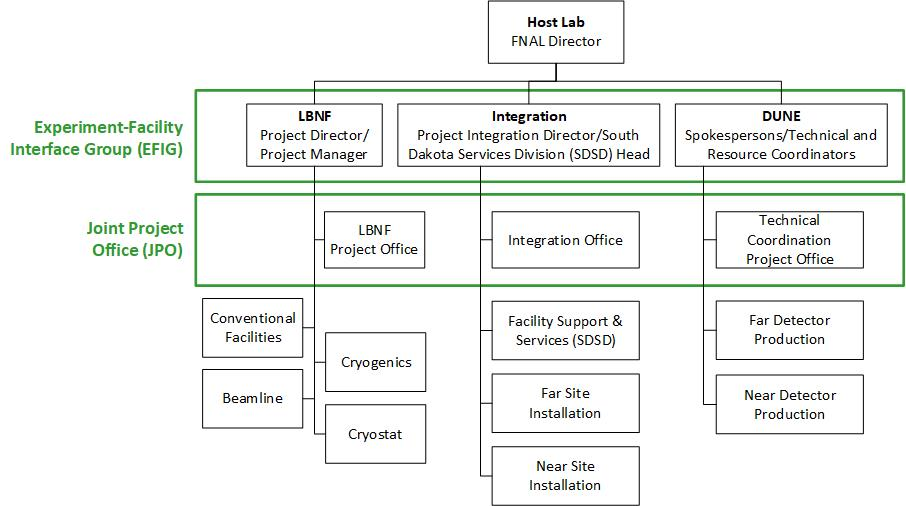
\includegraphics[width=0.95\textwidth]{FS_Integration_OrgChart_notitle}
\end{dunefigure}

The overall
coordination of installation activities in the underground caverns 
is managed as a separate element of \dword{lbnf-dune} under the
responsibility of the \dword{ipd}, who is appointed by and reports
to the \dword{fnal} director.  To ensure coordination across
all elements of \dword{lbnf-dune}, the \dword{ipd} connects to both
the facilities and detector construction projects through ex-officio
positions on the \dword{lbnf} project management board and
\dword{dune} \dword{exb}, respectively.  The \dword{ipd} receives support from the \dword{sdsd},
a \dword{fnal} division established to 
provide the necessary supporting infrastructure for installation, commissioning, and operation 
of the \dword{dune} far detector. 
%The \dword{dune} consortia maintain responsibility for the installation and commissioning of their detector subsystems and  \dword{lbnf} retains responsibility for the installation and commissioning of supporting infrastructure items.  --- already said

%\subsection{EFIG}
The \dword{efig} is the body responsible for the required high-level
coordination between the \dword{lbnf} and \dword{dune} construction 
projects. 
The \dword{efig} is augmented by the \dword{jpo} that supports both 
the \dword{lbnf} and \dword{dune} projects as well as the integration
effort that connects the two together. The \dword{jpo} combines
project support functions that exist within the different elements 
of the global project to ensure proper coordination across the entire 
\dword{lbnf-dune} enterprise.  Project functions coordinated globally 
through the \dword{jpo} are shown in Figure~\ref{fig:DUNE_jpo} along 
with the team members %personnel 
currently supporting these functions  %The team members who support these functions 
within the \dword{jpo} framework. 
These team members are drawn from the \dword{lbnf} project office, \dword{dune} \dword{tc}, 
and \dword{lbnf-dune} \dword{integoff} personnel.  
\begin{dunefigure}[JPO functions]{fig:DUNE_jpo}
  {\dword{jpo} global support functions and teams}
  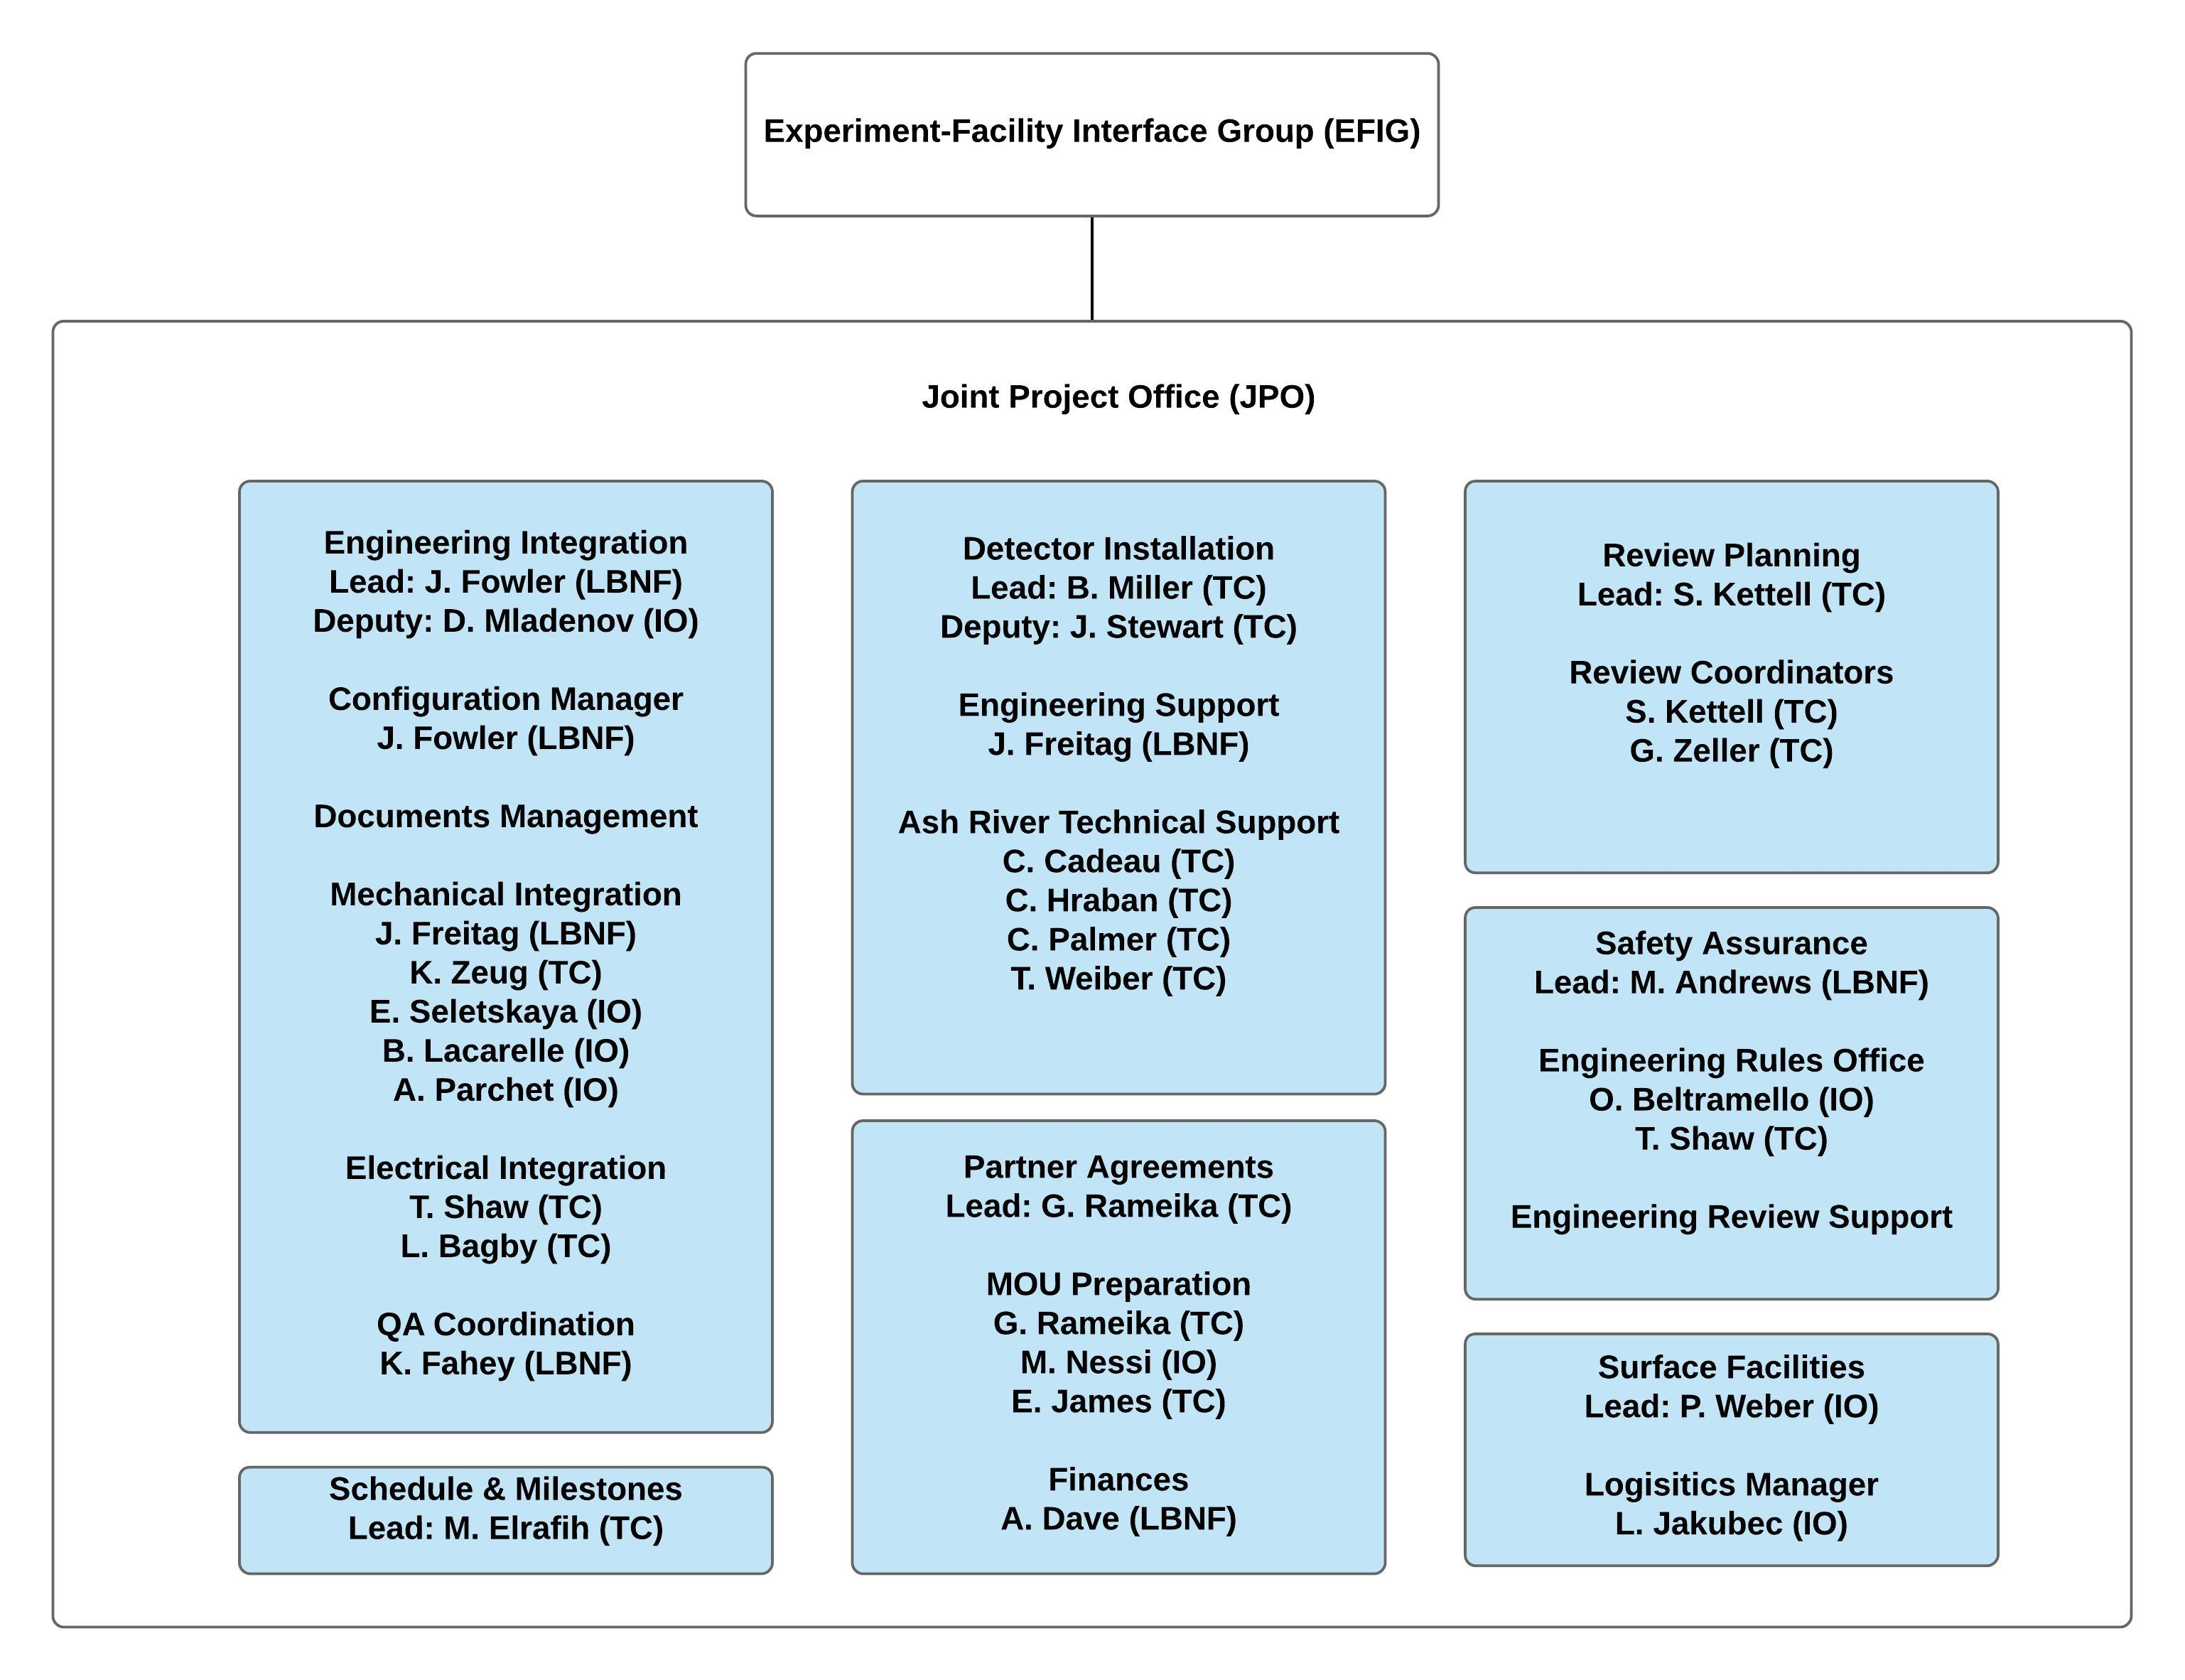
\includegraphics[width=0.85\textwidth]{JPO_OrgChart_v4}
\end{dunefigure}


\subsection{Coordinated Global Project Functions}

Project support functions requiring \dword{jpo} coordination include
safety, engineering integration, change control and document 
management, scheduling, review planning and oversight, and development 
of partner agreements.  

Planning activities related to detector installation and the provision 
of surface facilities are also currently embedded within the framework 
of the \dword{jpo} to ensure that all project elements are properly 
incorporated.  At the time when \dword{lbnf} \dword{fscf} delivers 
\dword{aup} of the underground detector caverns at \dword{surf}, the 
coordination of on-site activities associated with detector installation 
and the operation of surface facilities will be fully embedded within 
the \dword{lbnf}/\dword{dune} \dword{integoff} under the direction of the \dword{ipd}.  

%%%

\subsection{Coordinated Safety Program}    
\label{sec:dune_safety}


To ensure a consistent approach to safety across \dword{lbnf-dune},
a single \dword{lbnf-dune} \dword{esh} manager reports 
to the \dword{lbnf} project director, the \dword{ipd}, and \dword{dune}
management (via the \dword{dune} \dword{tcoord}).  This individual
directs separate safety teams responsible for implementing the
\dword{lbnf-dune} \dword{esh} program within %both 
the individual \dword{lbnf} 
and \dword{dune} projects as well as the coordinated \dword{lbnf}/\dword{dune}
installation activities at \dword{surf}. The safety organization 
is shown in Figure~\ref{fig:dune_esh}.

\begin{dunefigure}[\dshort{lbnf-dune} \dshort{esh}]{fig:dune_esh}
  {High level \dword{lbnf-dune} \dword{esh} organization.}
  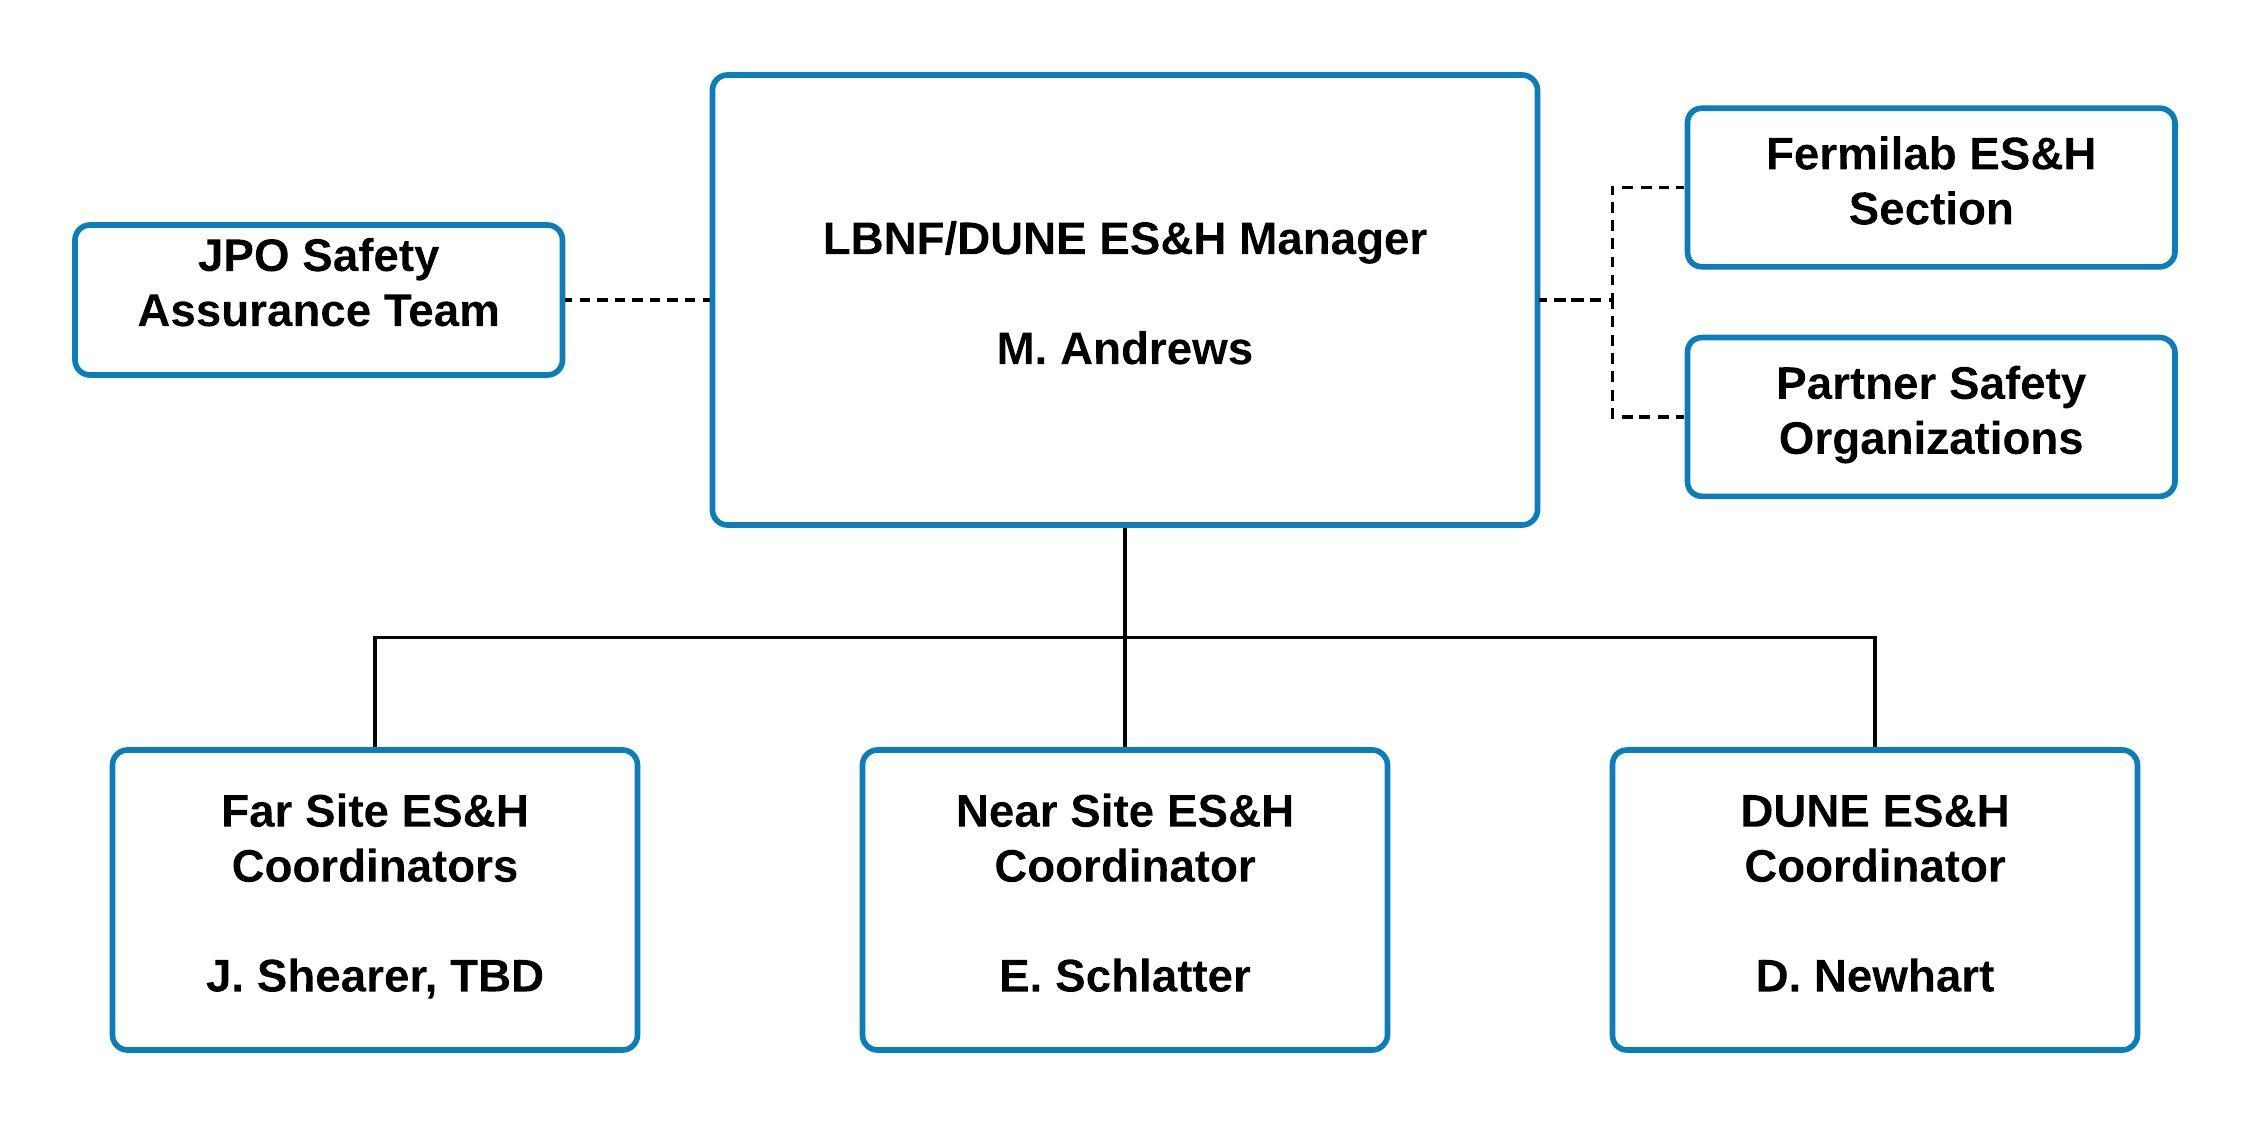
\includegraphics[width=0.85\textwidth]{DUNE_Safety_Org_Chart_v2}
\end{dunefigure}
The \dword{lbnf-dune} \dword{esh} manager works with the \dword{fnal} 
and \dword{surf} safety organizations to ensure that all project-related 
activities comply with the rules and regulations of the host 
organizations.  

The \dword{jpo} engineering safety assurance team defines a common 
set of design and construction rules (mechanical and electrical) to 
ensure consistent application of engineering standards and engineering 
documentation requirements across \dword{lbnf-dune}.  
Following lessons learned from the processes used for the 
\dword{protodune} detectors, an important mandate of the engineering 
safety assurance team is to ensure that safety issues related to 
component handling and installation are incorporated within the 
earliest stages of the design review process.  

\subsection{%Engineering 
Detector Integration}   
\label{sec:dune_engineering}


A central \dword{jpo} engineering team is responsible for building 
an integrated model of the detectors within their supporting
infrastructure and the \dword{fscf} that house them.  %The \dword{jpo} 
This team incorporates approved changes as they 
are received and checks to ensure that no errors or space conflicts 
are introduced into the model.    After receiving the appropriate sign-offs from all 
parties, the %\dword{jpo} 
team tags a new frozen release of the model 
and makes it available to the design teams as the current release 
against which the next set of design changes will be generated.

Electrical engineers are incorporated within %the central \dword{jpo} 
this team to ensure proper integration of the detector electrical 
components. 

The \dword{jpo} engineering team is also responsible for documenting and
controlling the interfaces between the \dword{lbnf} and \dword{dune} 
projects as well as the interfaces between these projects and the 
\dword{lbnf}/\dword{dune}  installation activities at \dword{surf}.  

The \dword{lbnf-dune} project partners have agreed to adopt 
the formal change control process developed previously for the 
\dword{lbnf} project.  The change control process applies to 
proposed modifications of requirements, technical designs, 
schedule, overall project scope, and assigned responsibilities 
for individual scope items. 

\subsection{Schedule and Milestones}   % done
\label{sec:dune_schedule}

The \dword{jpo} team is responsible for creating a single project
schedule for \dword{lbnf-dune} that incorporates all \dword{lbnf} and
\dword{dune} activities together with the installation activities at
\dword{surf}, incorporating all interdependencies.  This schedule
will be used to track the status of the global enterprise.   %Non-\dword{doe} activities will not be 
%tracked using the formal \dword{evms} procedures required for the 
%\dword{doe} project activities, but rather through regular assessments 
%of progress towards completion by the management teams responsible 
%for those activities. 
\dword{doe} activities will be 
tracked using the formal \dword{evms} procedures required for the 
\dword{doe} project activities; non-\dword{doe} activities will be tracked through regular assessments 
of progress towards completion by the management teams responsible 
for those activities. 



\subsection{Partner Agreements and Financial Reporting}   % done
\label{sec:dune_agreements}

Partner contributions to all project elements will be detailed 
in a series of written agreements.  In the case of \dword{lbnf}, 
these contributions will be spelled out in bilateral agreements 
between the \dword{doe} and each of the contributing partners.  In 
the case of \dword{dune},  a \dword{mou} will 
detail the contributions of all participating partners.  
A series of more technical agreements describing the exact 
boundaries between partner contributions and the terms and 
conditions under which they will be delivered will %lie just beneath 
accompany the primary agreements.  


%%%%%%%%%%%%%%%%%%%%%%%%%%%%%%%%%%%%%%%%%%%%%
\section{DUNE Far Detector Organization}   % done
%%%%%%%%%%%%%%%%%%%%%%
\subsection{Detector Design and Construction}   % done
\label{sec:es-tc-det-const}

The \dword{dune} \dword{fd} construction project refers collectively 
to the activities associated with the design and construction of 
necessary detector components.  \dword{dune} collaboration management 
is responsible for overseeing this portion of  \dword{lbnf-dune} and 
ensuring its successful execution.  The high-level \dword{dune} 
collaboration management team consisting of the co-spokespersons, 
\dword{tcoord}, and \dword{rcoord} is responsible for the
management of the construction project.  

Construction of the \dword{fd} modules is carried out by 
consortia of collaboration institutions who assume responsibility 
for detector subsystems.  Each consortium plans and executes the 
construction, installation, and commissioning of its subsystem.

%Management of each consortium is through 
Each consortium is managed by an overall consortium leader 
and a technical lead.  The consortium leader chairs an institutional 
board composed of one representative from each of the %collaborating 
institutions contributing to the activities of the consortium.  Major 
consortium decisions such as technology selections and assignment of 
responsibilities %within 
among the institutions %should 
pass  through its institutional board.  These decisions are then passed 
as recommendations to the \dword{dune} \dword{exb} for formal collaboration approval.

Because the consortia operate as self-managed entities, a strong
\dfirst{tc} organization is required to ensure overall integration 
of the detector elements and successful execution of the detector
construction project.  \Dword{tc} areas of responsibility include 
general project oversight, systems engineering, \dword{qa}, and 
safety.  \Dword{tc} also supports the planning and execution 
of integration and installation activities at \dword{surf}.
The \dword{tcoord} manages the overall detector construction 
project through regular technical and project board meetings with 
the consortium leadership teams and members of the \dword{tc} 
organization.

The \dword{tc} organization, headed by the \dword{tcoord}, supports the work of 
the consortia and has responsibility for a number of major project 
support functions prior to the delivery of detector components to 
\dword{surf}, including
\begin{itemize}
\item ensuring that each consortium has a well defined and complete
  scope, that interactions between consortia are sufficiently 
  well defined, and that any missing scope outside of the 
  consortia is provided through other sources such as collaboration
  common funds;
\item defining and documenting scope boundaries and technical 
  interfaces both between consortia and with \dword{lbnf};  
\item developing an overall schedule with appropriate dependencies
  between activities covering all phases of the project; 
\item ensuring that appropriate engineering and safety standards 
  are developed, understood, and agreed to by all key stakeholders 
  and that these standards are conveyed to and understood by each
  consortium;
\item ensuring that all \dword{dune} requirements on \dword{lbnf} 
  for \dword{fscf}, cryostat, and cryogenics are clearly defined and 
  agreed to by each consortium;
\item ensuring that each consortium has well developed and reviewed
  component designs, construction plans, \dword{qc} processes, and 
  safety programs; and
\item monitoring the overall project schedule and the progress of 
  each consortium towards delivering its assigned scope. 
\end{itemize}
The \dword{dune} \dword{tc} organizational structure is shown 
in Figure~\ref{fig:DUNE_tc}. 
\begin{dunefigure}[DUNE technical coordination organization]{fig:DUNE_tc}
  {\dword{dune} \dfirst{tc} organizational chart.}
  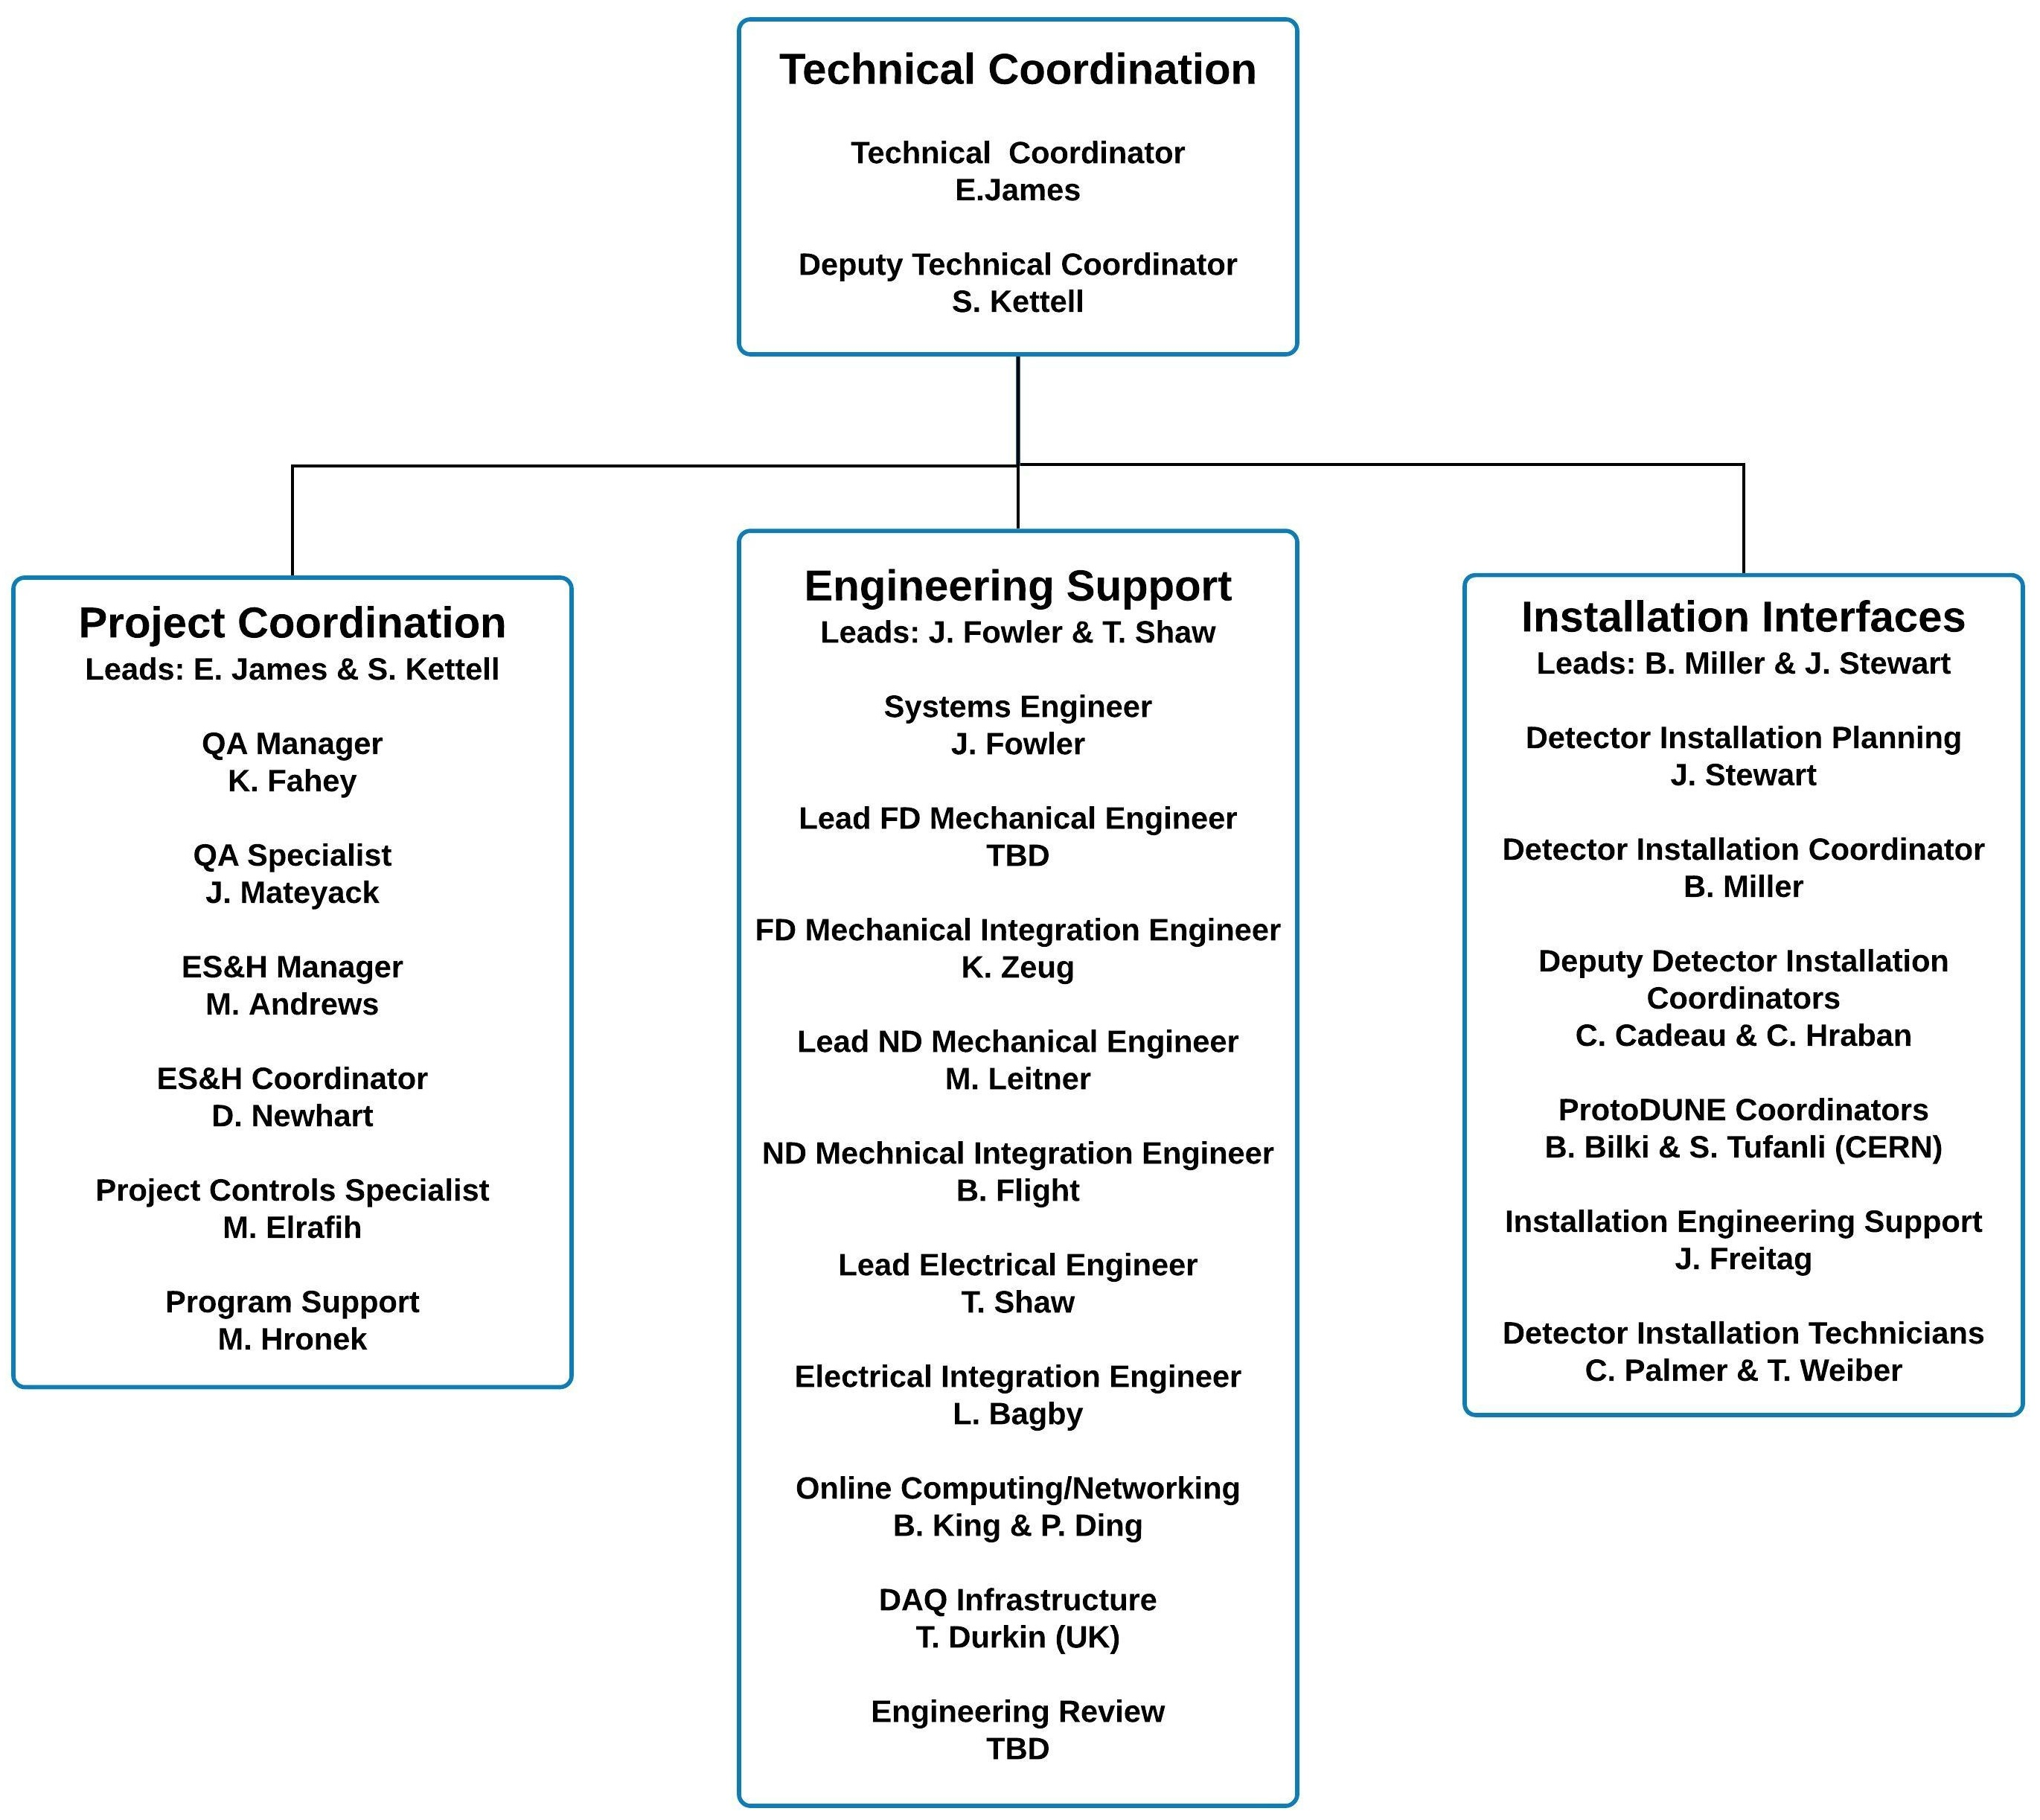
\includegraphics[width=0.99\textwidth]{TC_OrgChart_v2}
\end{dunefigure}

The \dword{tc} project coordination team incorporates \dword{esh}, 
\dword{qa}, and project controls specialists.  Overall integration 
of the detector elements is coordinated through the \dword{tc} 
engineering support team headed by the \dword{lbnf-dune} systems 
engineer and lead \dword{dune} electrical engineer.  Planning 
coordinators for integration and installation activities at 
\dword{surf} (who sit within the \dword{lbnf-dune} \dword{integoff}) also head the \dword{tc} installation interfaces team.  
The dual placement of these individuals facilitates the required 
coordination of integration and installation planning efforts between 
the core team directing these activities and the \dword{dune} 
consortia. %, which maintain primary responsibility for the individual detector subsystems. 

%%%%%%%%%%%%%%%%%%%%%%%%%%%%%%%%%%%%%%%%%%%%%
\subsection{Detector Installation and Commissioning}  % done 
\label{sec:es-tc-det-instal}

The \dfirst{ipd} has
responsibility for coordinating the planning and execution of 
the \dword{lbnf-dune} installation activities, both 
in the underground detector caverns at \dword{surf} and in 
nearby surface facilities. 

The \dword{lbnf-dune} \dword{integoff} will evolve over 
time to incorporate the team in South Dakota responsible for the 
overall coordination of on-site installation activities.  In the 
meantime, the installation planning team within the \dword{integoff} works with 
the \dword{dune} consortia and \dword{lbnf} project team members 
to plan these activities.  This installation team is responsible for specification 
and procurement of common infrastructure items associated with 
installation of the detectors. 
The organization of the on-site team is 
shown in Figure~\ref{fig:io-org-chart}. 

\begin{dunefigure}[Integration office installation team org chart]{fig:io-org-chart}
  {\Dword{integoff} installation team organization chart}
  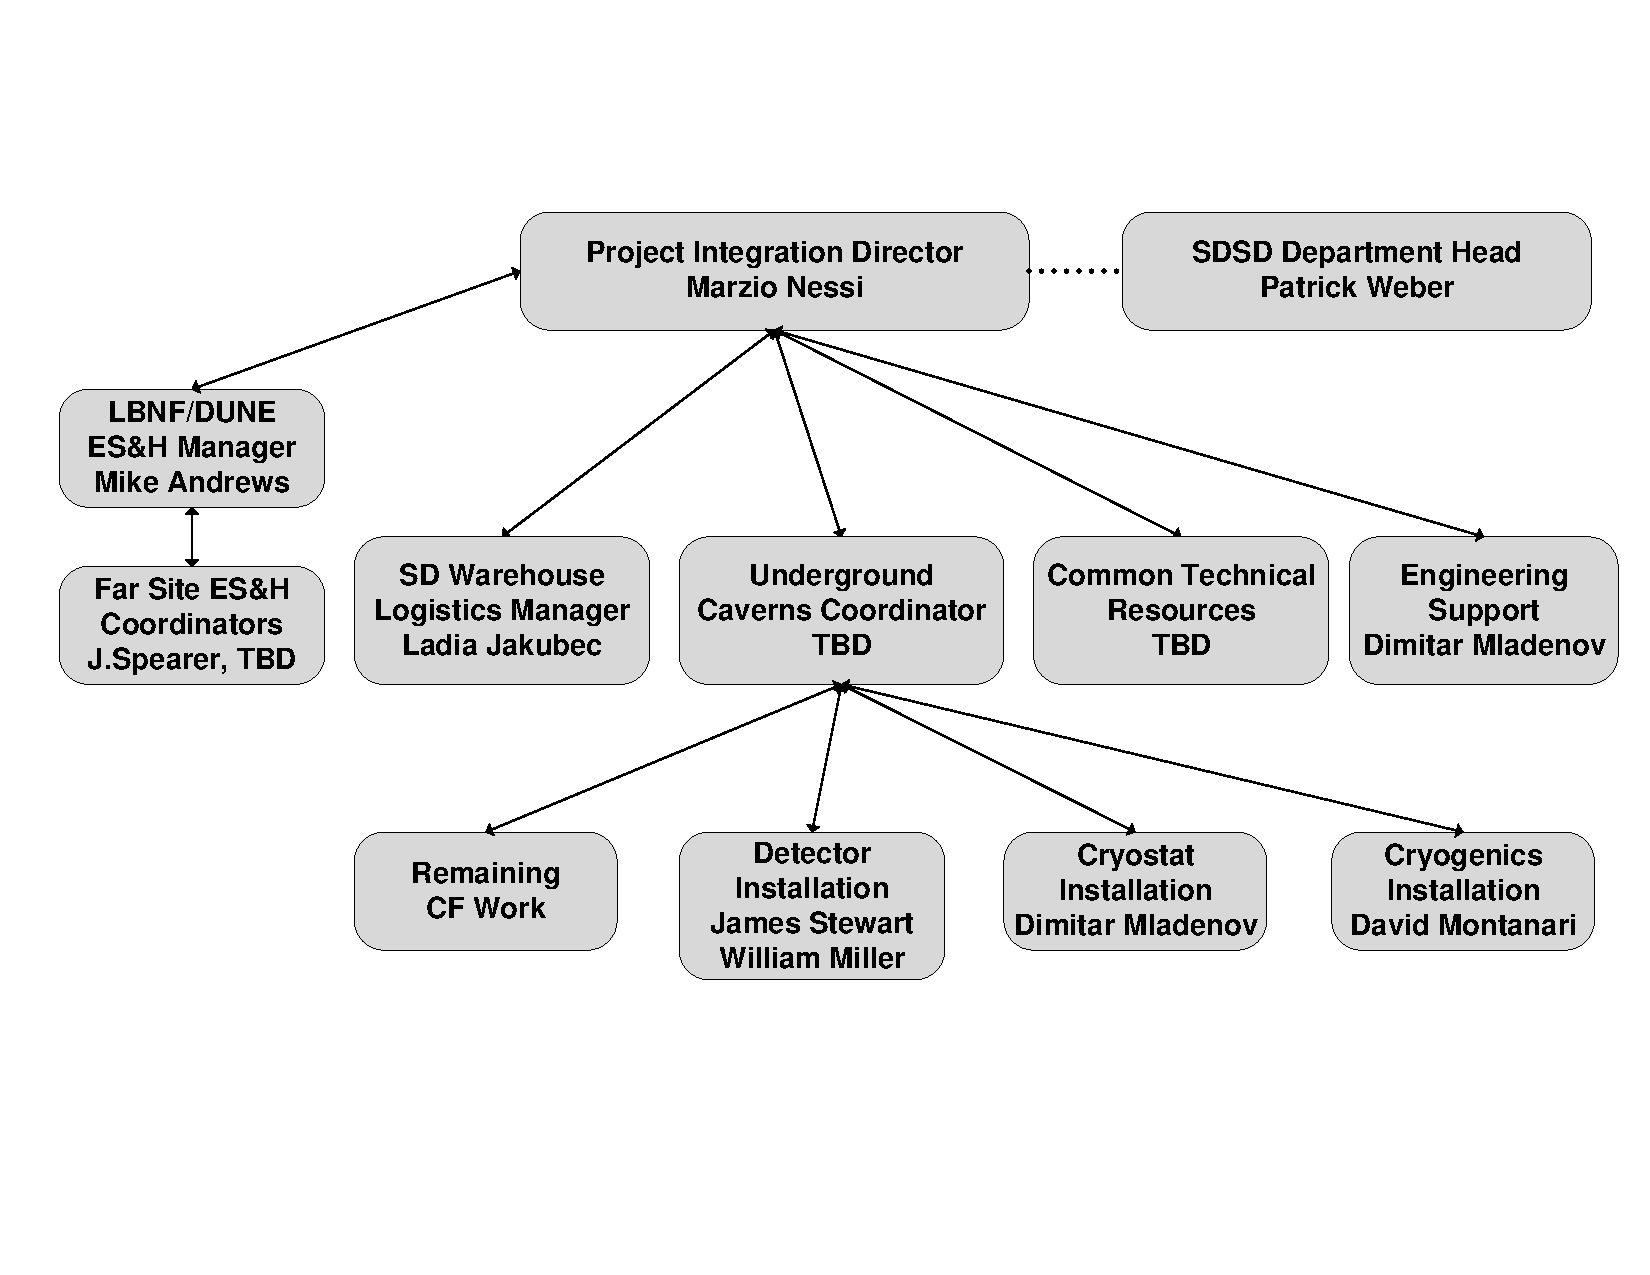
\includegraphics[width=0.95\textwidth]{org-farsite-io.pdf}
\end{dunefigure}


The full on-site \dword{integoff} team includes rigging teams responsible for moving 
materials in and out of the shaft, through the underground drifts, 
and within the detector caverns, and personnel responsible 
for overseeing safety and logistics planning. 

The underground caverns coordinator is responsible for managing all 
activities in the two underground detector caverns and the
\dword{cuc}. The detector installation teams, distinct from the \dword{integoff}  installation team, 
incorporate a substantial number of scientific and
technical personnel from the \dword{dune} consortia.  \Dword{integoff} coordinators 
of the detector installation effort are jointly placed within 
\dword{dune} \dword{tc} to facilitate consortia involvement in  
detector installation activities.  Any modifications to the facilities 
occurring after \dword{aup} are managed by the underground cavern 
coordinator under the direction of the \dword{ipd}.

The \dword{lbnf-dune}
\dword{esh} manager heads the on-site safety organization and reports
to the \dword{ipd} to support the execution of this
responsibility. The far site \dword{esh} coordinators %sitting under the \dword{lbnf-dune} \dword{esh} manager 
oversee the day-to-day execution
of the installation work.

%%%%%%%%%%%%%%%%%%%%%%%%%%%%%%%%%%%%%%%%%%%%%
\section{Facility Description}
\label{sec:es-tc-facility}

The \dword{dune} underground campus at the \dword{surf} 4850L is shown in
Figures~\ref{fig:caverns} and~\ref{fig:dune-underground}. The primary path for both personnel 
and material access to the underground excavations is through the Ross Shaft.
\begin{dunefigure}[Underground campus]{fig:dune-underground}
  {Underground campus at the 4850L.}
  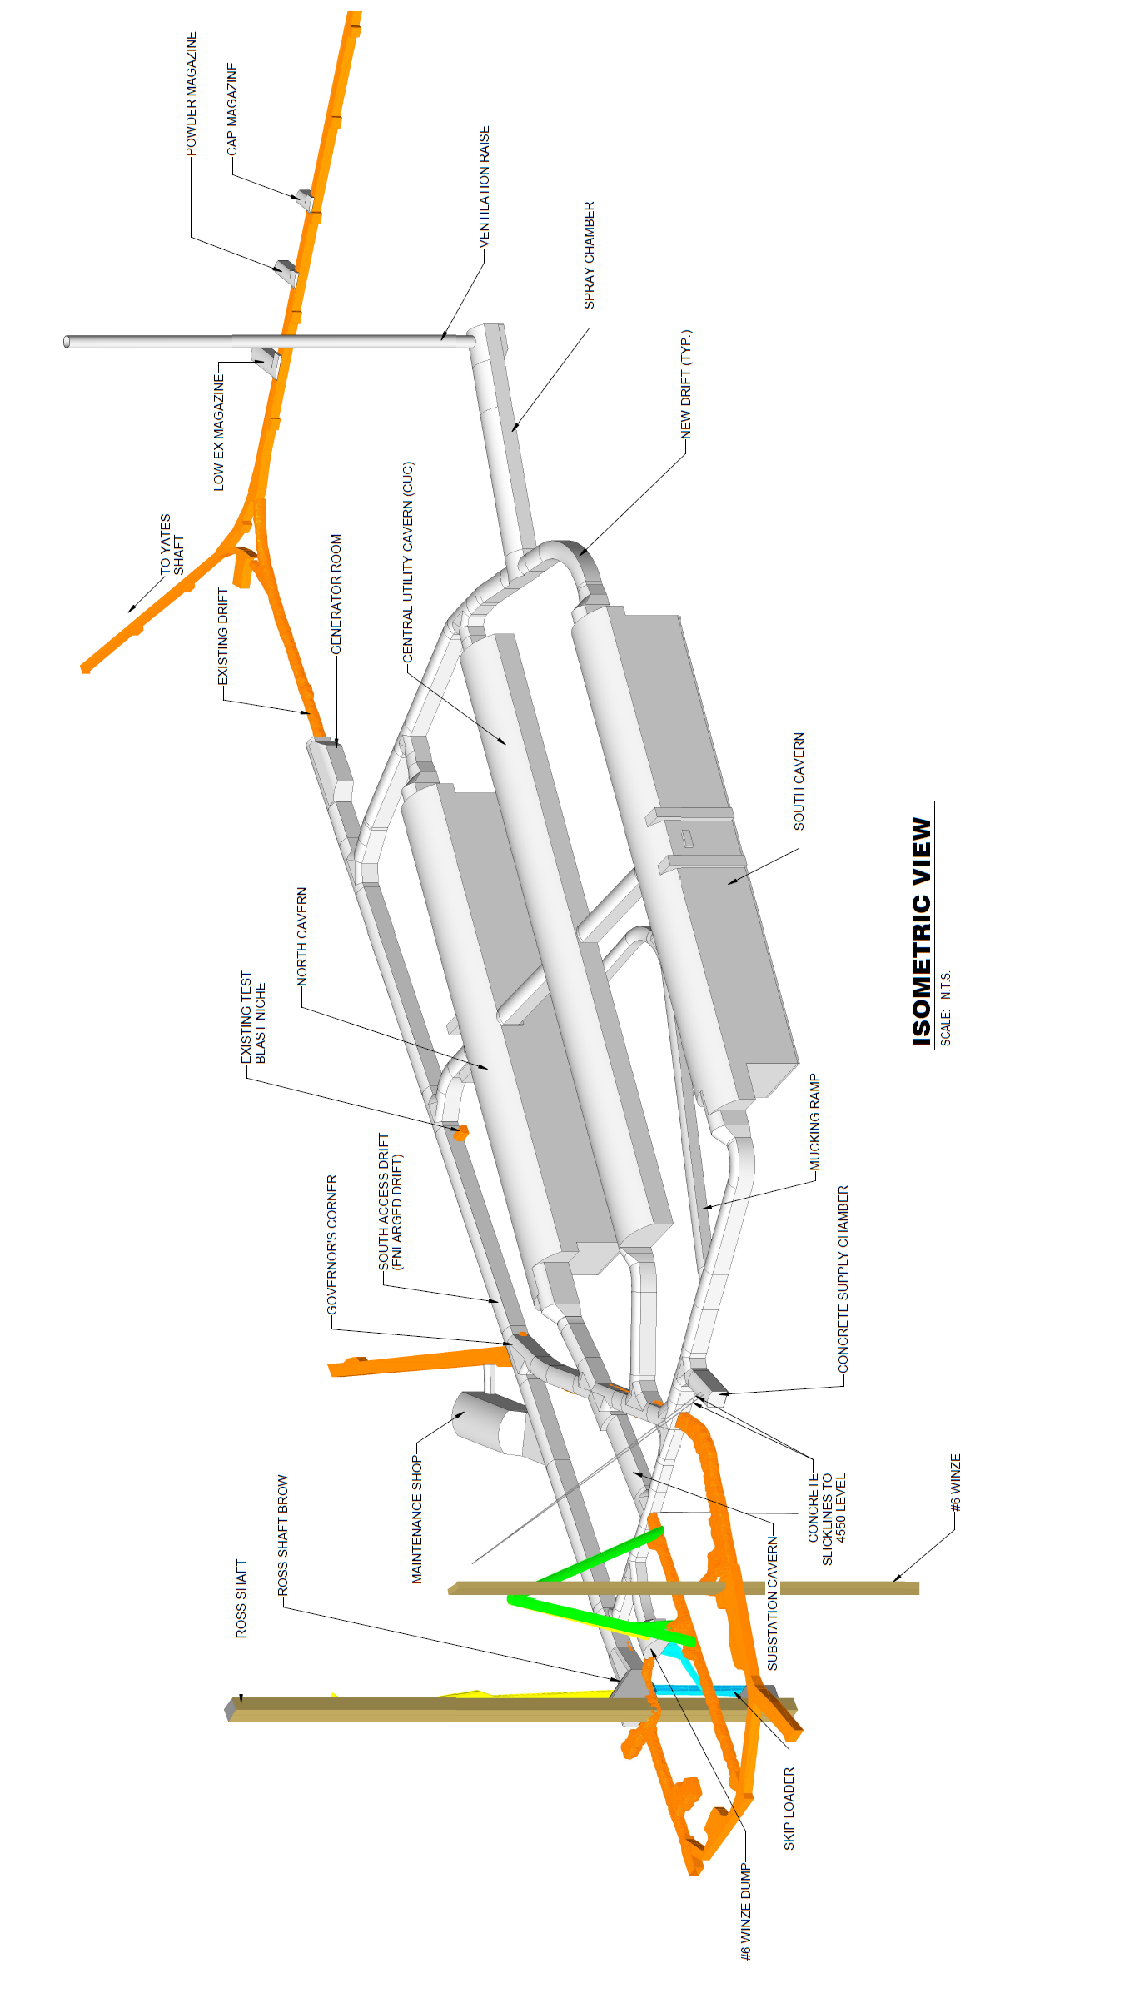
\includegraphics[width=0.75\textwidth]{underground_campus_vertical}
\end{dunefigure}

\dword{lbnf} will provide facilities and services, on the surface and
underground, to support the \dword{dune} \dword{fd}.  This includes
logistical, cryogenics, electrical, mechanical, cyber, and environmental
facilities and services.  All of these facilities are provided for the
safe and productive operation of the \dwords{detmodule}.

On the surface, a new compressor building is being constructed
adjacent to the Ross headframe.  This building will house the cryogenics
systems for receiving cryogenic fluids and preparing them for delivery
down the Ross Shaft.  New piping is being installed down the 
shaft compartment to transport \dword{gar} and nitrogen underground
where they will be reliquefied.


Two large detector caverns
are being excavated.  Each of these caverns will support two
\larmass{}-capacity cryostats.  The caverns, labeled north and
south, are \SI{144.5}{\meter} long, \SI{19.8}{\meter} wide,  and 
%\SI{27.95}{\meter} 
\SI{28.0}{\meter} high. The tops of the cryostats are approximately
aligned with the 4850L of \dword{surf}, with the bottoms resting
at the 4910L.  A \SI{12}{\meter} space between the cryostats will
be used %as part of 
for the detector installation process, for placement of
cryogenic pumps and valves, and for access to the 4910L.  The
\dword{cuc}, between the north and south caverns, is \SI{190}{\meter}
long, \SI{19.3}{\meter} wide, and \SI{10.95}{\meter} high. 

The \dword{sdwf} is planned as a leased \SI{5000}{\square\meter} facility, hosted by 
\dword{sdsd}, to be located within a maximum one-day roundtrip of \dword{surf}.  
It must be in place for receiving cryostat and detector 
components approximately six months before \dword{aup}
of the underground detector caverns is received. 
 Laydown space near the Ross headframe is extremely 
limited.  For this reason, the transportation of materials from 
the \dword{sdwf} to the top of the Ross shaft requires careful 
coordination. The \dword{lbnf-dune} logistics manager works 
with the \dword{cmgc} through the end of excavation activities  
and with other members of the \dword{integoff} team to coordinate transport 
of materials into the underground areas.  Since no detector materials or 
equipment can be shipped directly to \dword{surf}, %the Ross or Yates headframes, 
the \dword{sdwf} will be used for both short- and long-term storage, as 
well as for any re-packaging of items required prior to transport 
into the underground areas. 


%%%%%%%%%%%%%%%%%%%%%%%%%%%%%%%%%%%%%%%%%%%%%
\section{Far Detector Construction Management}
\label{sec:es-tc-det-mgmt}


Eleven \dword{fd} consortia have been formed to cover 
the subsystems required for the \dword{sp} and \dword{dp} detector technologies  (Figure~\ref{fig:DUNE_consortia}). % currently underconsideration.  
%In particular, t
Three consortia (SP-APA, SP-TPC
Electronics and SP-Photon Detection) pursue subsystems specific to
the \dword{sp} design and another three consortia (DP-CRP, DP-TPC
Electronics, and DP-Photon Detection) pursue designs for \dword{dp}-specific 
subsystems.  %An additional f
Five consortia (HV System, \dword{daq},
\dword{cisc}, Calibration, and Computing)
have responsibility for subsystems common to both detector
technologies.    

\begin{dunefigure}[DUNE far detector consortia]{fig:DUNE_consortia}
  {Consortia associated with the \dword{fd} construction effort along with their 
current leadership teams. CL refers to consortium leader
    and TL refers to technical lead.}
  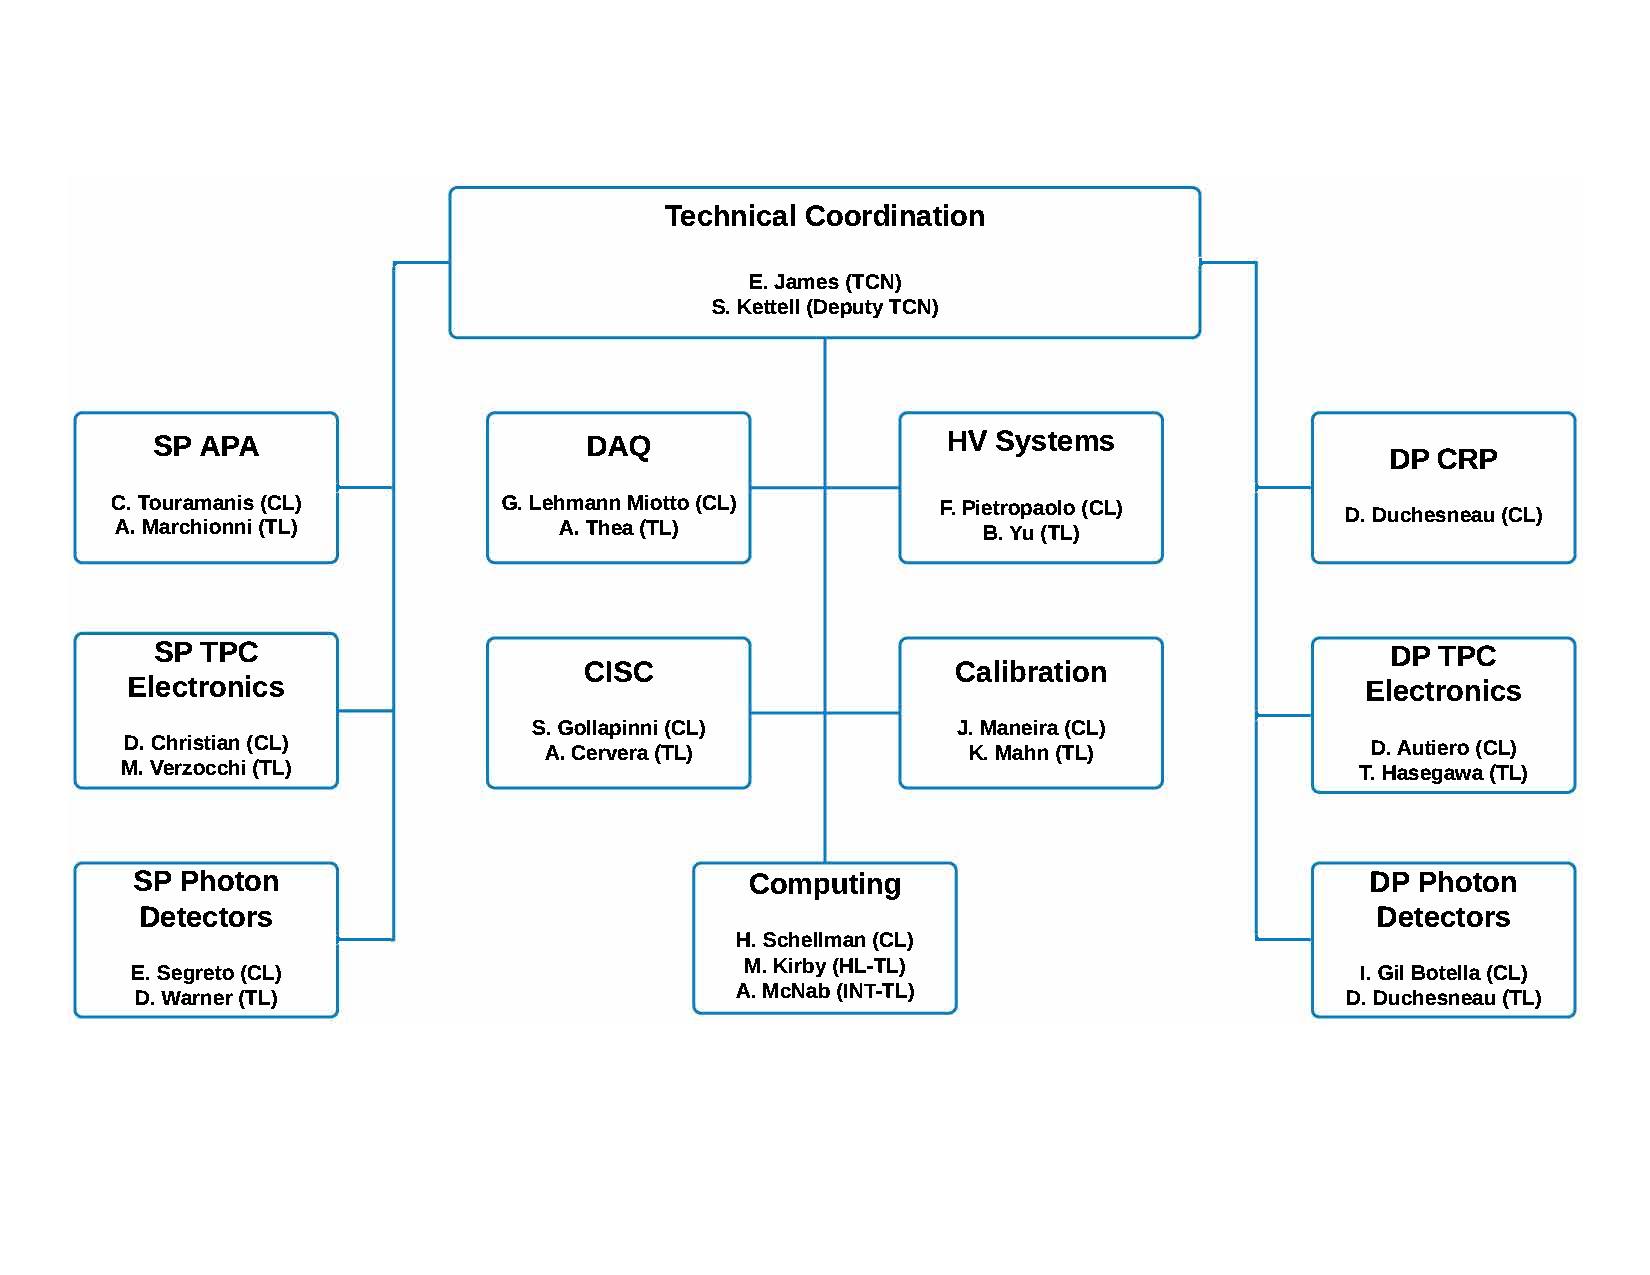
\includegraphics[width=0.99\textwidth]{Consortia_Org_Chart}
\end{dunefigure}

The complete scope of the \dword{dune} construction project is captured in a 
\dword{wbs} to define and document the distribution of deliverables among 
the consortia.  In combination with interface documentation, the 
\dword{wbs} is used to validate that all necessary scope is covered.  The 
\dword{wbs} is also used as a framework for building \dword{dune} 
detector cost estimates.

The highest-level layers of the \dword{dune} \dword{wbs} are summarized 
in Figure~\ref{fig:WBS_level2}.  At level 1 the \dword{wbs} is broken down into 
six elements, which correspond to \dword{tc} (TC in the figure), %the five \dword{dune} detector modules (
four 
\dword{fd} modules, and a \dword{nd}.  The scope documented %here 
in this \dword{tdr} is fully contained within the elements of level-1 items 1 through 3, the \dword{tc}, a \dword{sp} \dword{fd} module, and a \dword{dp} \dword{fd} module.

\begin{dunefigure}[DUNE WBS at level 2]{fig:WBS_level2}
  {High level \dword{dune} \dword{wbs} to level 2.}
  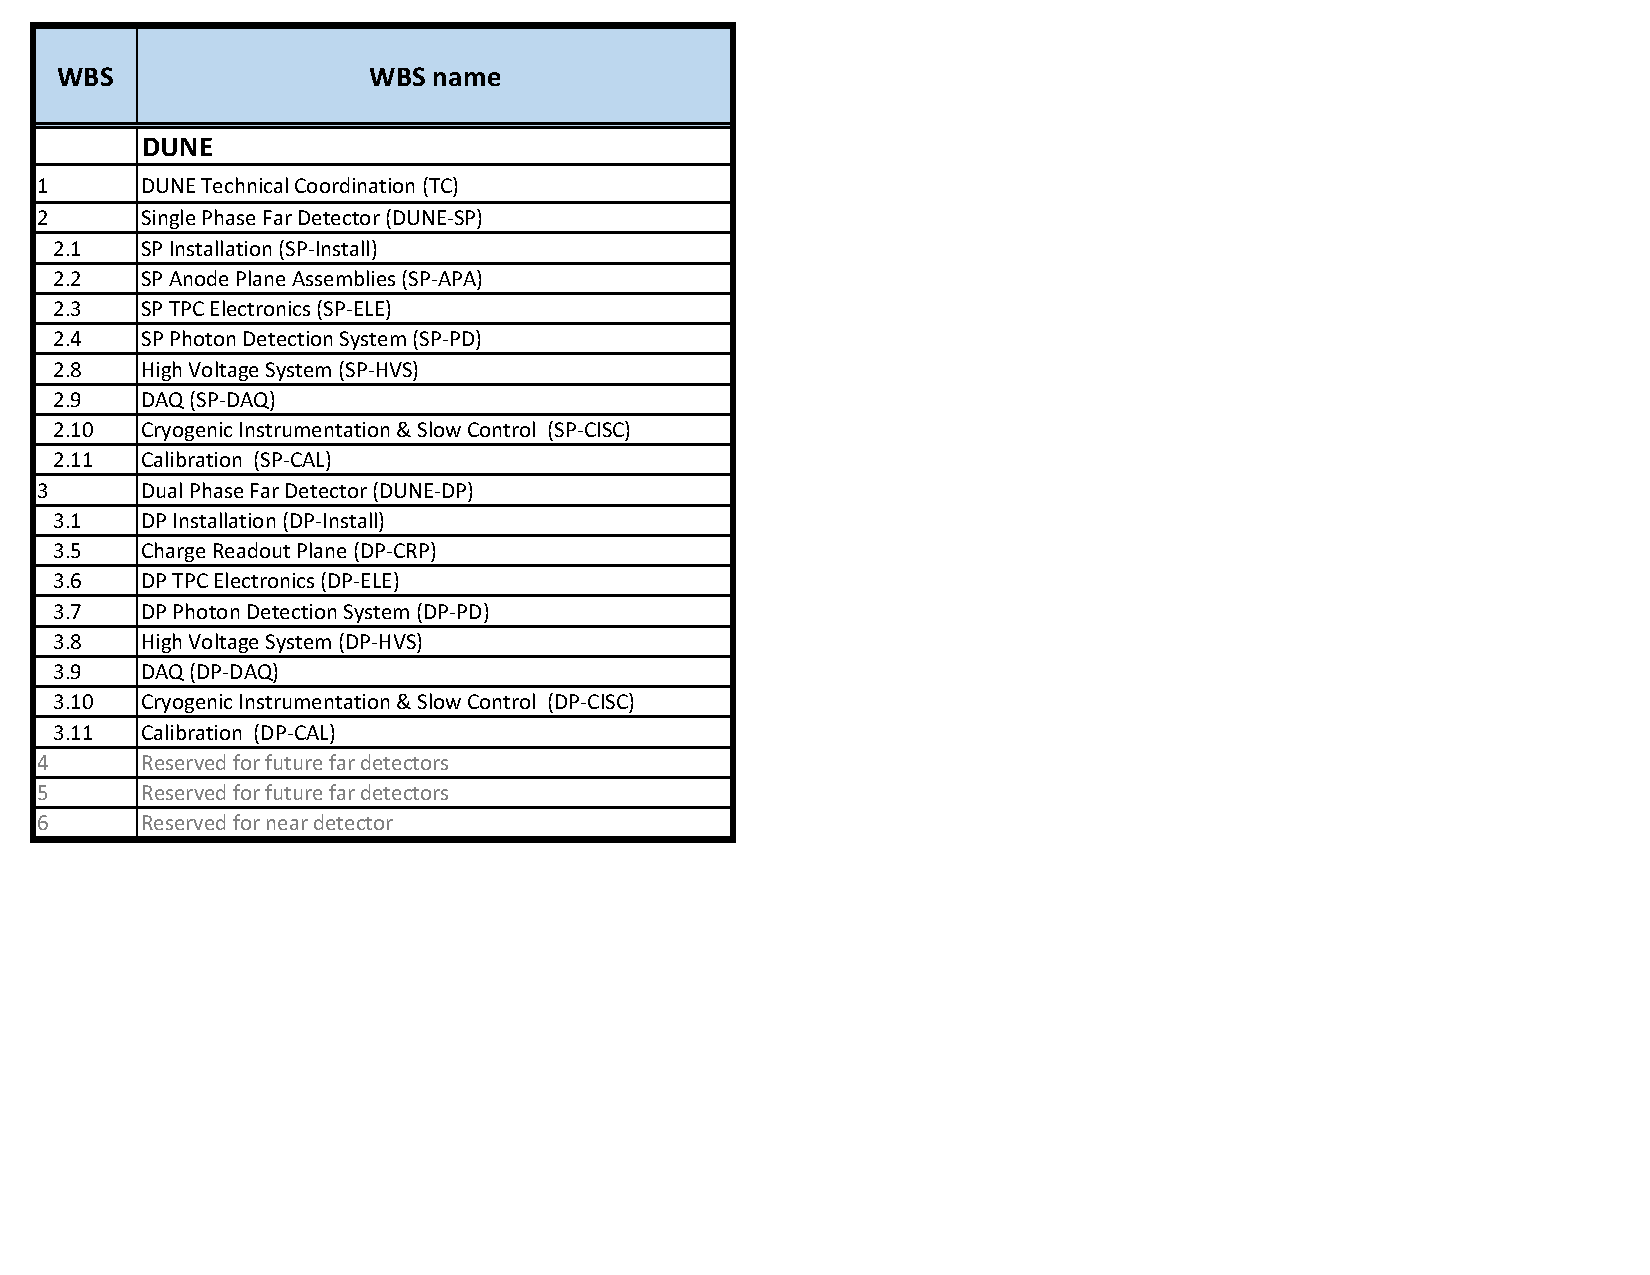
\includegraphics[width=0.75\textwidth]{WBS_level2_v2}
\end{dunefigure}

%%%%%%%%%%%%%%%%%%%%%%%%%%%%%%%%%%%%%%%%%%%%%
\section{Integration Engineering}
\label{sec:es-coord-integ-sysengr}

Integration engineering for \dword{dune} encompasses three principal focus areas. First, it %focuses on configuring the
covers configuration of the mechanical and electrical systems of each \dword{detmodule} and management of 
the interfaces within them; this includes verifying that subassemblies
and their interfaces %are built 
conform to the approved design of each detector element.
%e.g., \dword{apa} or \dword{pds}. The second major focus 
A second area is assurance that the \dwords{detmodule} can be integrated and
installed into their final configurations. Third, it covers %The third major focus is
integration of the necessary services provided by \dword{fscf} 
with the \dwords{detmodule}. The overall effort involves 
%To this end, t
the \dword{jpo} engineering team, who maintains
subsystem component documentation for detector
configuration management, and 
the consortia, who provide engineering data for their detector subsystems to the \dword{jpo} team for incorporation into the global configuration files.


An integration mechanism has been developed to manage and create an
overall model of interfaces both within a \dword{detmodule} and
between a \dword{detmodule} and facilities. The mechanism defines
integration nodes, %which can be thought of as focus areas.  The 
between which the \dword{jpo} engineering team carries out and
manages interfaces. % between the nodes. 
Figure~\ref{fig:integration_nodes} shows the interfaces and nodes between a
\dword{detmodule} and the facilities it requires. The \dword{jpo} engineering
team also ensures that the interfaces are appropriately defined
and managed for the \dword{daq} room in the \dword{cuc} and the surface
control and network rooms. Interfaces with \dword{lbnf}
are managed at the boundaries of each integration node.  
Interface documents are developed and maintained to manage the
interfaces between consortia and between each consortium and 
\dword{lbnf}.


\begin{dunefigure}[Integration nodes and interfaces]{fig:integration_nodes}
  {Overall integration nodes and interfaces. The items
provided by \dword{lbnf} within the cavern are shown on the left and the items provided by
\dword{dune} are on the right.}
  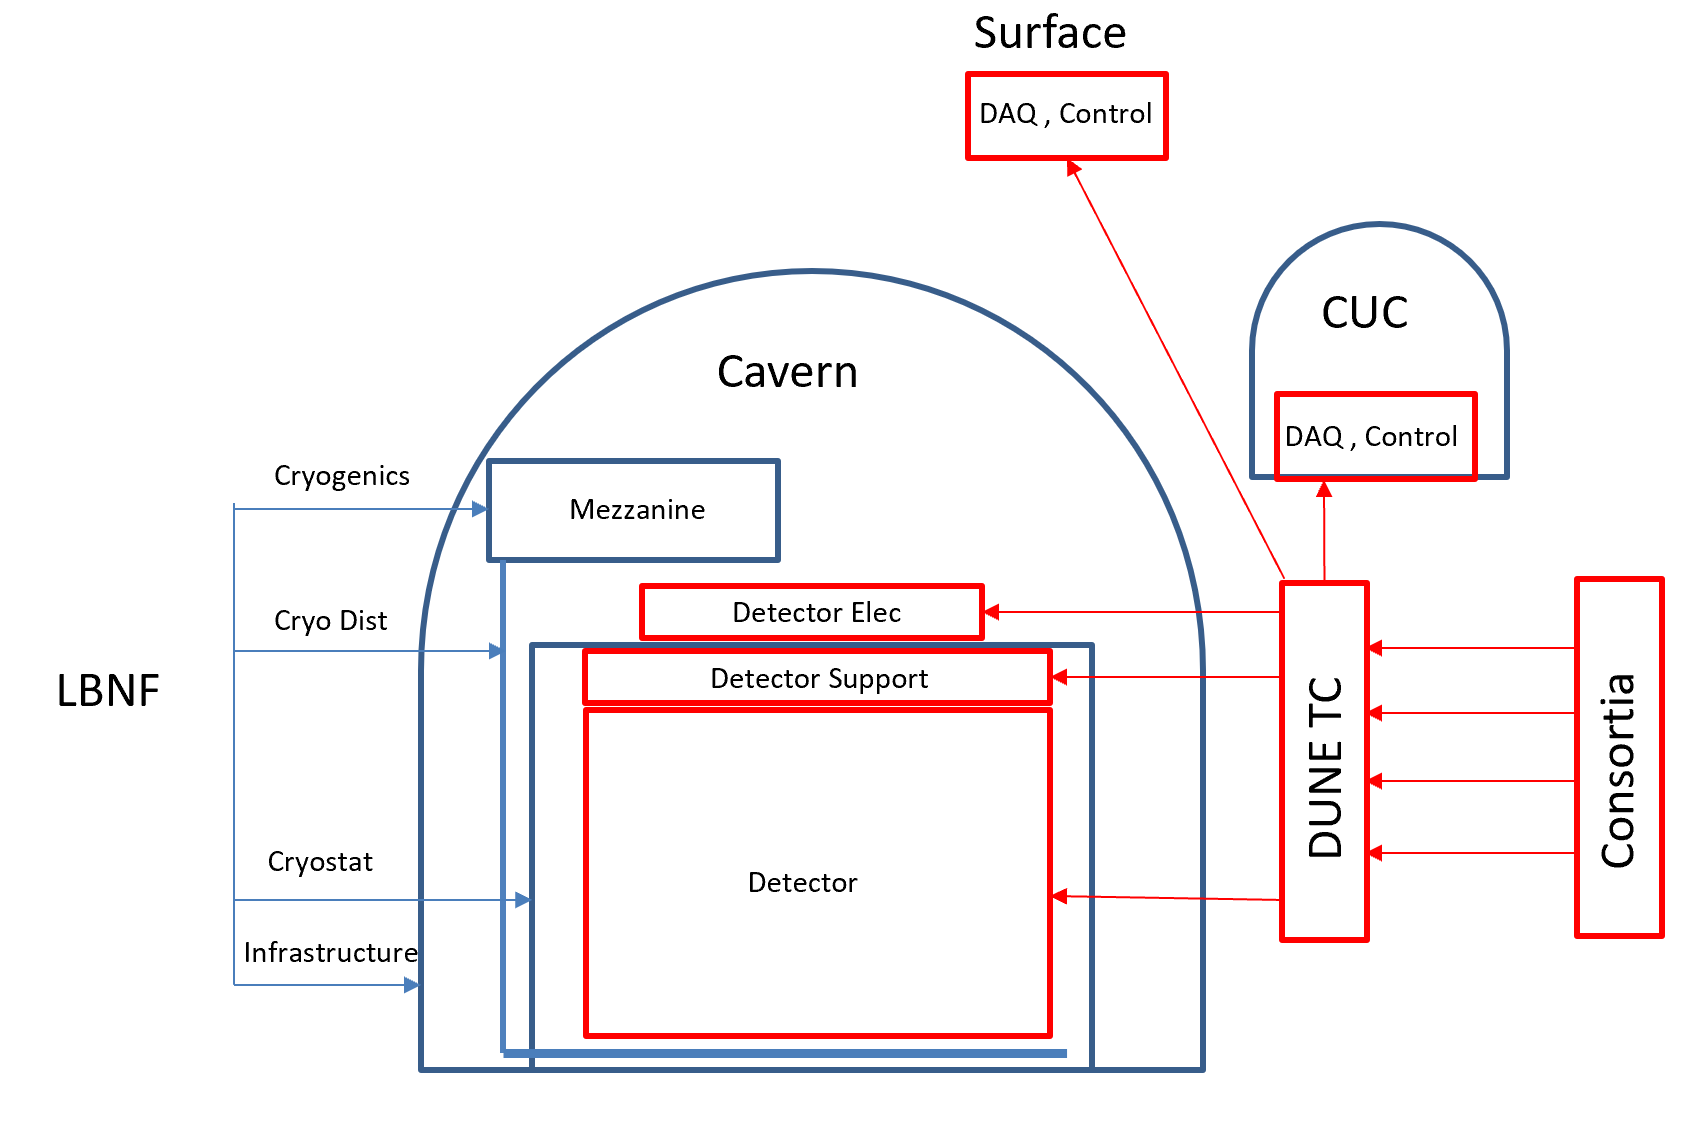
\includegraphics[width=0.7\textwidth]{Integration_nodes.png}
\end{dunefigure}




%%%%%%%%%%%%%%%%%%%%%%%%%%%%%%%%%%%%%%%%%%%%%
\section{Reviews}
\label{sec:es-tc-reviews}

The \dword{integoff} and \dword{tc} review all stages of detector development
and work with each consortium to arrange reviews of the design
(\dword{cdrev}, \dword{pdr} and \dword{fdr}), production (\dword{prr}
and \dword{ppr}), installation (\dword{irr}), and operation
(\dword{orr}) of their system. The reviews are organized by the
\dword{jpo} \dword{ro}.  These
reviews provide information to the \dword{tb}, \dword{exb}, and \dword{efig}
in evaluating technical decisions. 

Review reports are tracked by the \dword{jpo} \dword{ro} and \dword{tc} and provide
guidance on key issues that require engineering oversight by the
\dword{jpo} engineering team. The \dword{ro}  maintains a
calendar of \dword{dune} reviews. 

%%%%%%%%%%%%%%%%%%%%%%%%%%%%%%%%%%%%%%%%%%%%%
\section{Quality Assurance}
\label{sec:es-tc-qa}

\dshort{dune} \dword{tc} monitors technical contributions from
collaborating institutions and provides centralized project
coordination functions. One part of this project coordination is
standardizing \dfirst{qa}/\dfirst{qc} practices, a facet
of which is to assist consortia in defining and implementing
\dword{qa}/\dword{qc} plans that maintain uniform, high
standards across the entire detector construction
effort. Figure~\ref{fig:fnal_qa} shows how \dword{dune} \dword{tc}
derives its \dword{qa} program from the principles of the \fnal \dword{qa} program:
requirements %are flowed 
flow down through the \dword{lbnf-dune}
\dword{qa} program into the \dword{qc} plans developed for consortium fabrication of
detector components and integration and installation of the detector.
\begin{dunefigure}[Quality assurance flowdown]{fig:fnal_qa}
  {Flow-down of \fnal \dword{qa} to consortia}
  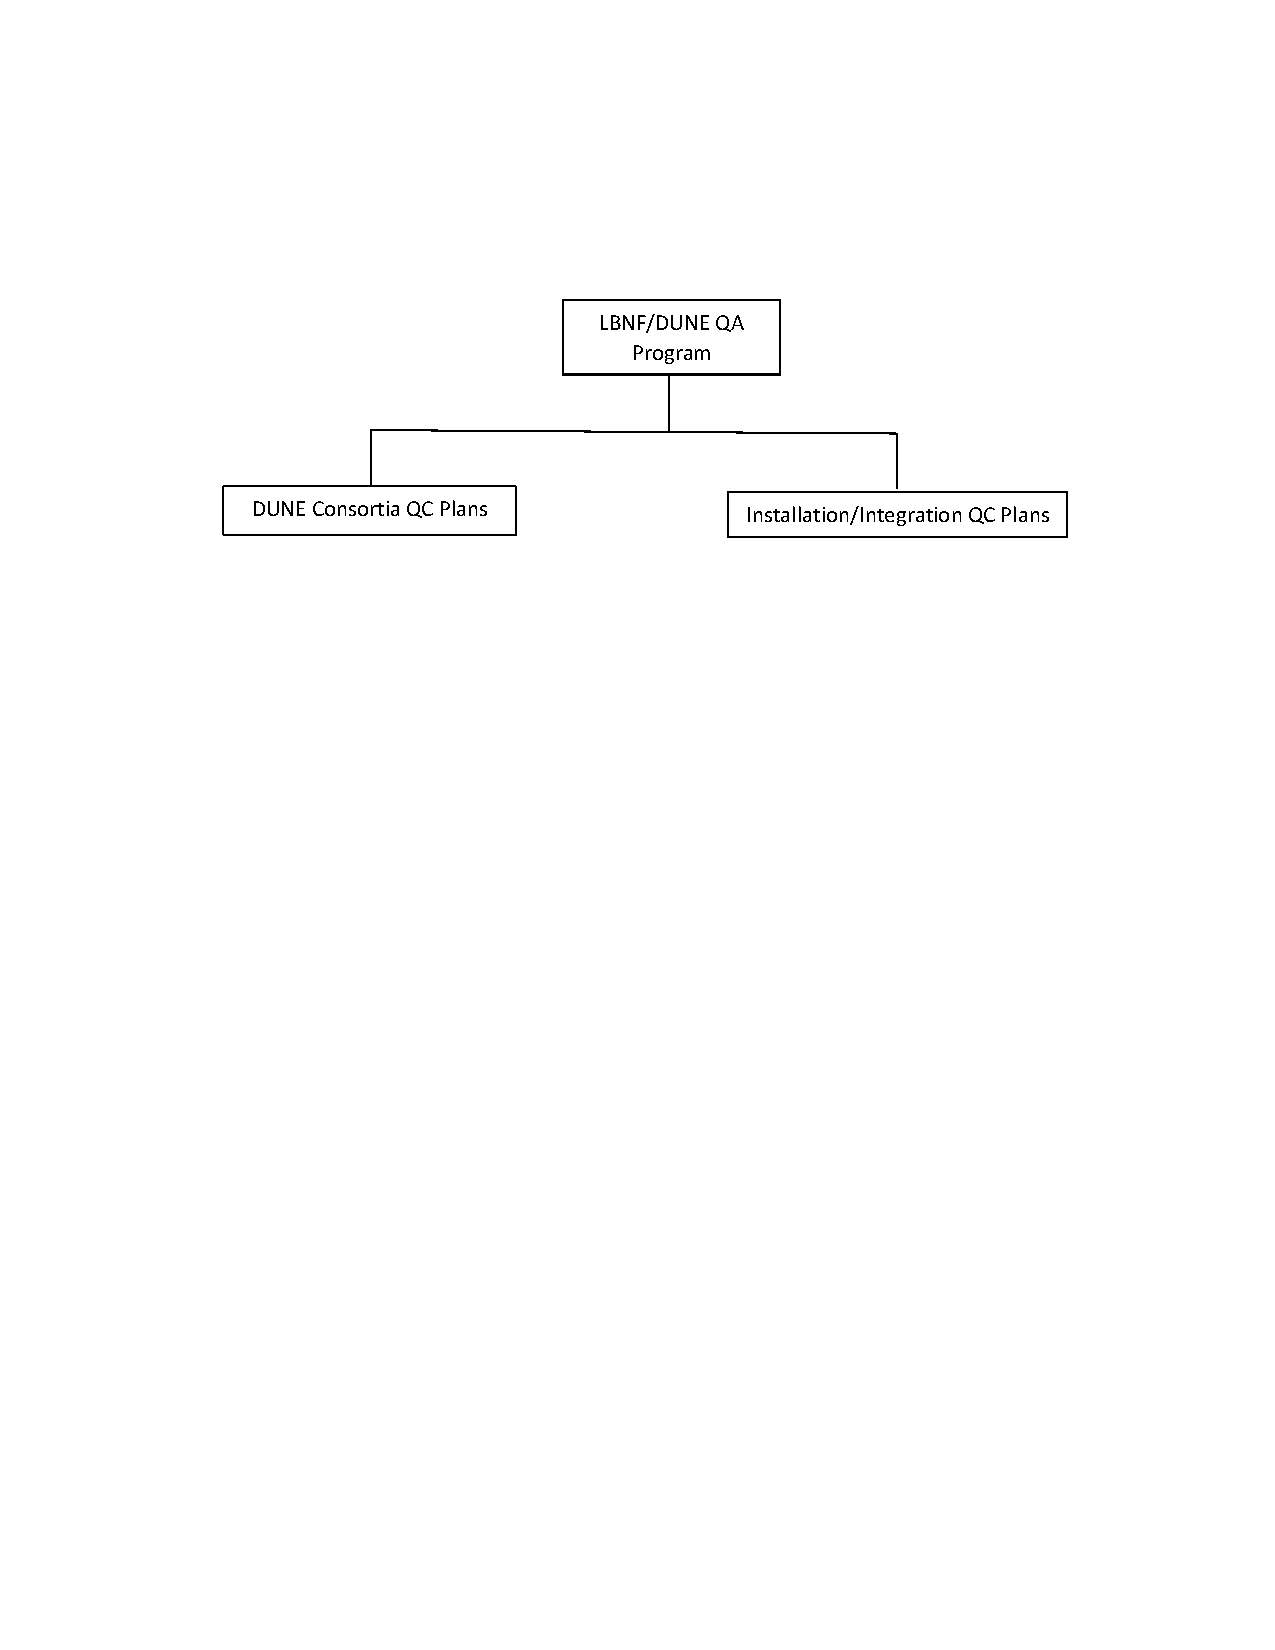
\includegraphics[width=0.85\textwidth]{fnal_qa.pdf}
\end{dunefigure}
The \dword{qa} effort includes design, production readiness, and
progress reviews as appropriate for the \dword{dune} detector
subsystems, as was done for \dword{pdsp} under \dword{tc}
oversight.

The primary objective of the \dword{lbnf-dune} \dword{qa} program is
to assure quality in the construction of the \dword{lbnf} facility and
\dword{dune} experiment while providing protection of
\dword{lbnf-dune} personnel, the public, and the environment. The
\dword{qa} plan aligns \dword{lbnf-dune} \dword{qa} activities, which
are spread around the world, with the principles of the \dword{fnal} Quality
Assurance Manual. The manual identifies the \dword{fnal} Integrated Quality
Assurance Program features that serve as the basis for the
\dword{lbnf-dune} \dword{qa} plan.

A key element of the \dword{lbnf-dune} \dword{qa} plan is the
concept of graded approach; that is, applying a level of analysis,
controls, and documentation commensurate with the potential for an
environmental, safety, health, or quality impact. To promote continuous improvement, \dword{dune} \dword{tc} will develop a
lessons learned program based on the \dword{fnal} Office of Project Support
Services lessons learned program.


The \dword{qa} plan
defines the \dword{qa} roles and responsibilities of the \dword{dune}
project. The \dword{dune} consortium leaders are responsible for identifying the
resources to ensure that their team members are adequately trained and
qualified to perform their assigned work.
All consortium members are responsible for the quality of the work that
they do and for using guidance and assistance that is available. All
have the authority to stop work and report adverse conditions that
affect quality of \dword{dune} products to their respective
\dword{dune} consortium leader and the \dword{lbnf-dune}
\dword{qa} manager.




%%%%%%%%%%%%%%%%%%%%%%%%%%%%%%%%%%%%%%%%%%%%%
\section{Environment, Safety, and Health}
\label{sec:es-tc-eshq}

\dword{lbnf-dune} is committed to protecting the health and safety of
staff, the community, and the environment, as stated in the
\dword{lbnf-dune} integrated \dword{esh} plan~\cite{bib:docdb291}.

The \dword{lbnf-dune} \dword{esh} program complies with applicable
standards and local, state, federal, and international legal
requirements through the \dword{fnal} Work Smart set of standards and the
contract between \dword{fra} and the \dword{doe}
Office of Science (FRA-DOE). \dword{fnal}, as the host laboratory,
established the \dword{sdsd} to provide facility support.
\dword{sdsd} is responsible for support of \dword{lbnf-dune}
operations at \dword{surf}.

The \dword{tcoord} and \dword{ipd} have responsibility for
implementation of the \dword{dune} \dword{esh} program for the construction and installation activities, respectively.  The
\dword{lbnf-dune} \dword{esh} manager reports to the
\dword{tcoord} and \dword{ipd} and is responsible for providing
\dword{esh} support and oversight for development and implementation of the 
\dword{lbnf-dune} \dword{esh} program. 

The \dword{dune} \dword{esh} coordinator reports to the
\dword{lbnf-dune} \dword{esh} manager and has primary responsibility
for \dword{esh} support and oversight of the \dword{dune} \dword{esh}
program for activities at collaborating institutions.  The far and near site
\dword{esh} coordinators are responsible for providing daily field support and
oversight for all installation activities at the \dword{surf}
and \dword{fnal} sites.

The \dword{lbnf-dune} \dword{esh} plan defines the \dword{esh}
requirements applicable to installation activities at the \dword{surf}
site. A key element of an effective \dword{esh} program is the hazard
identification process. Hazard identification allows production of a
list of hazards within a facility, so these hazards can be screened
and managed through a suitable set of controls. All work activities
are subject to work planning and \dword{ha}.  
All work planning documentation is reviewed and
approved by the \dword{dune} \dword{esh} coordinator and the \dword{dune}
\dword{irr} or \dword{orr} committees prior to the start of work activities.

A Safety Data Sheet (SDS) will be available for all chemicals and
hazardous materials that are used on-site. All chemicals and hazardous
materials brought to the \dword{surf} site must be reviewed and approved by the
\dword{dune} \dword{esh} coordinator and the \dword{surf} \dword{esh}
department before arriving at the site.

\dword{sdsta} will maintain an emergency response incident command
system and an emergency response team (\dword{ert}) on all shifts that can access the
underground sites with normal surface fire department response
times. This team provides multiple response capabilities for both
surface and underground emergencies.

Fire and life safety requirements for \dword{lbnf-dune} areas were
analyzed in the \dword{lbnf-dune} Far Site Fire and Life Safety
  Assessment. All caverns will be equipped with
fire detection and suppression systems, with both visual and audible
notification.  All fire alarms and system supervisory signals will be
monitored in the \dword{surf} Incident Command Center.  The
\dword{surf} \dword{ert} will respond with additional support from the
Lead and Deadwood Fire Departments and the county's emergency management
department. The caverns will be equipped with
an \dword{odh} monitoring and alarm system, with independent visual and
audible notification systems.

All workers on the \dword{dune} project have the
authority to stop work in any situation that presents an imminent
threat to safety, health, or the environment. Work may not resume
until the circumstances are investigated and the deficiencies corrected,
including the concurrence of the \dword{dune} \dword{ipd}
and \dword{lbnf-dune} \dword{esh} manager.

